%%%%%%%%%%%%%%%%%%%%%%%%%%%%%%%%%%%%%%%%%
% Beamer Presentation
% LaTeX Template
% Version 1.0 (10/11/12)
%
% This template has been downloaded from:
% http://www.LaTeXTemplates.com
%
% License:
% CC BY-NC-SA 3.0 (http://creativecommons.org/licenses/by-nc-sa/3.0/)
%
%%%%%%%%%%%%%%%%%%%%%%%%%%%%%%%%%%%%%%%%%

%----------------------------------------------------------------------------------------
%	PACKAGES AND THEMES
%----------------------------------------------------------------------------------------

\documentclass{beamer}

\mode<presentation> {

% The Beamer class comes with a number of default slide themes
% which change the colors and layouts of slides. Below this is a list
% of all the themes, uncomment each in turn to see what they look like.

%\usetheme{default}
%\usetheme{AnnArbor}
%\usetheme{Antibes}
%\usetheme{Bergen}
%\usetheme{Berkeley}
%\usetheme{Berlin}
%\usetheme{Boadilla}
%\usetheme{CambridgeUS}
%\usetheme{Copenhagen}
%\usetheme{Darmstadt}
%\usetheme{Dresden}
%\usetheme{Frankfurt}
%\usetheme{Goettingen}
%\usetheme{Hannover}
%\usetheme{Ilmenau}
%\usetheme{JuanLesPins}
%\usetheme{Luebeck}
\usetheme{Madrid}
%\usetheme{Malmoe}
%\usetheme{Marburg}
%\usetheme{Montpellier}
%\usetheme{PaloAlto}
%\usetheme{Pittsburgh}
%\usetheme{Rochester}
%\usetheme{Singapore}
%\usetheme{Szeged}
%\usetheme{Warsaw}

% As well as themes, the Beamer class has a number of color themes
% for any slide theme. Uncomment each of these in turn to see how it
% changes the colors of your current slide theme.

%\usecolortheme{albatross}
%\usecolortheme{beaver}
%\usecolortheme{beetle}
%\usecolortheme{crane}
%\usecolortheme{dolphin}
%\usecolortheme{dove}
%\usecolortheme{fly}
%\usecolortheme{lily}
%\usecolortheme{orchid}
%\usecolortheme{rose}
%\usecolortheme{seagull}
%\usecolortheme{seahorse}
%\usecolortheme{whale}
%\usecolortheme{wolverine}

%\setbeamertemplate{footline} % To remove the footer line in all slides uncomment this line
%\setbeamertemplate{footline}[page number] % To replace the footer line in all slides with a simple slide count uncomment this line

%\setbeamertemplate{navigation symbols}{} % To remove the navigation symbols from the bottom of all slides uncomment this line
}
\usepackage{xeCJK}
\usepackage{graphicx} % Allows including images
\usepackage{booktabs} % Allows the use of \toprule, \midrule and \bottomrule in tables

%----------------------------------------------------------------------------------------
%	TITLE PAGE
%----------------------------------------------------------------------------------------
\title[Business Strategy]{Mid-Pre: Case Analysis of \textbf{ZOOM}} % The short title appears at the bottom of every slide, the full title is only on the title page

\author{Group 2} % Your name
\institute[ENTR1006,Fall20] % Your institution as it will appear on the bottom of every slide, may be shorthand to save space
{
\textit{ZiyeLiu,YuweiMao,ChengShi,BoYang} % Your email address
}
\date{\today} % Date, can be changed to a custom date

\begin{document}

\begin{frame}
\titlepage % Print the title page as the first slide
\end{frame}

\begin{frame}
\frametitle{Overview} % Table of contents slide, comment this block out to remove it
\tableofcontents % Throughout your presentation, if you choose to use \section{} and \subsection{} commands, these will automatically be printed on this slide as an overview of your presentation
\end{frame}

%----------------------------------------------------------------------------------------
%	PRESENTATION SLIDES
%----------------------------------------------------------------------------------------

%------------------------------------------------
\section{Zoom's Strategy} % Sections can be created in order to organize your presentation into discrete blocks, all sections and subsections are automatically printed in the table of contents as an overview of the talk
%------------------------------------------------

%\subsection{Subsection Example} A subsection can be created just before a set of slides with a common theme to further break down your presentation into chunks



\begin{frame}
\frametitle{Zoom's Strategy}
\textcolor{blue}{Zoom recently entered conferencing hardware, describe the strategy using the framework (e.g. Arena, Differentiator, Staging/Pacing, Vehicles, Economic Logic).}
\begin{figure}[h]
    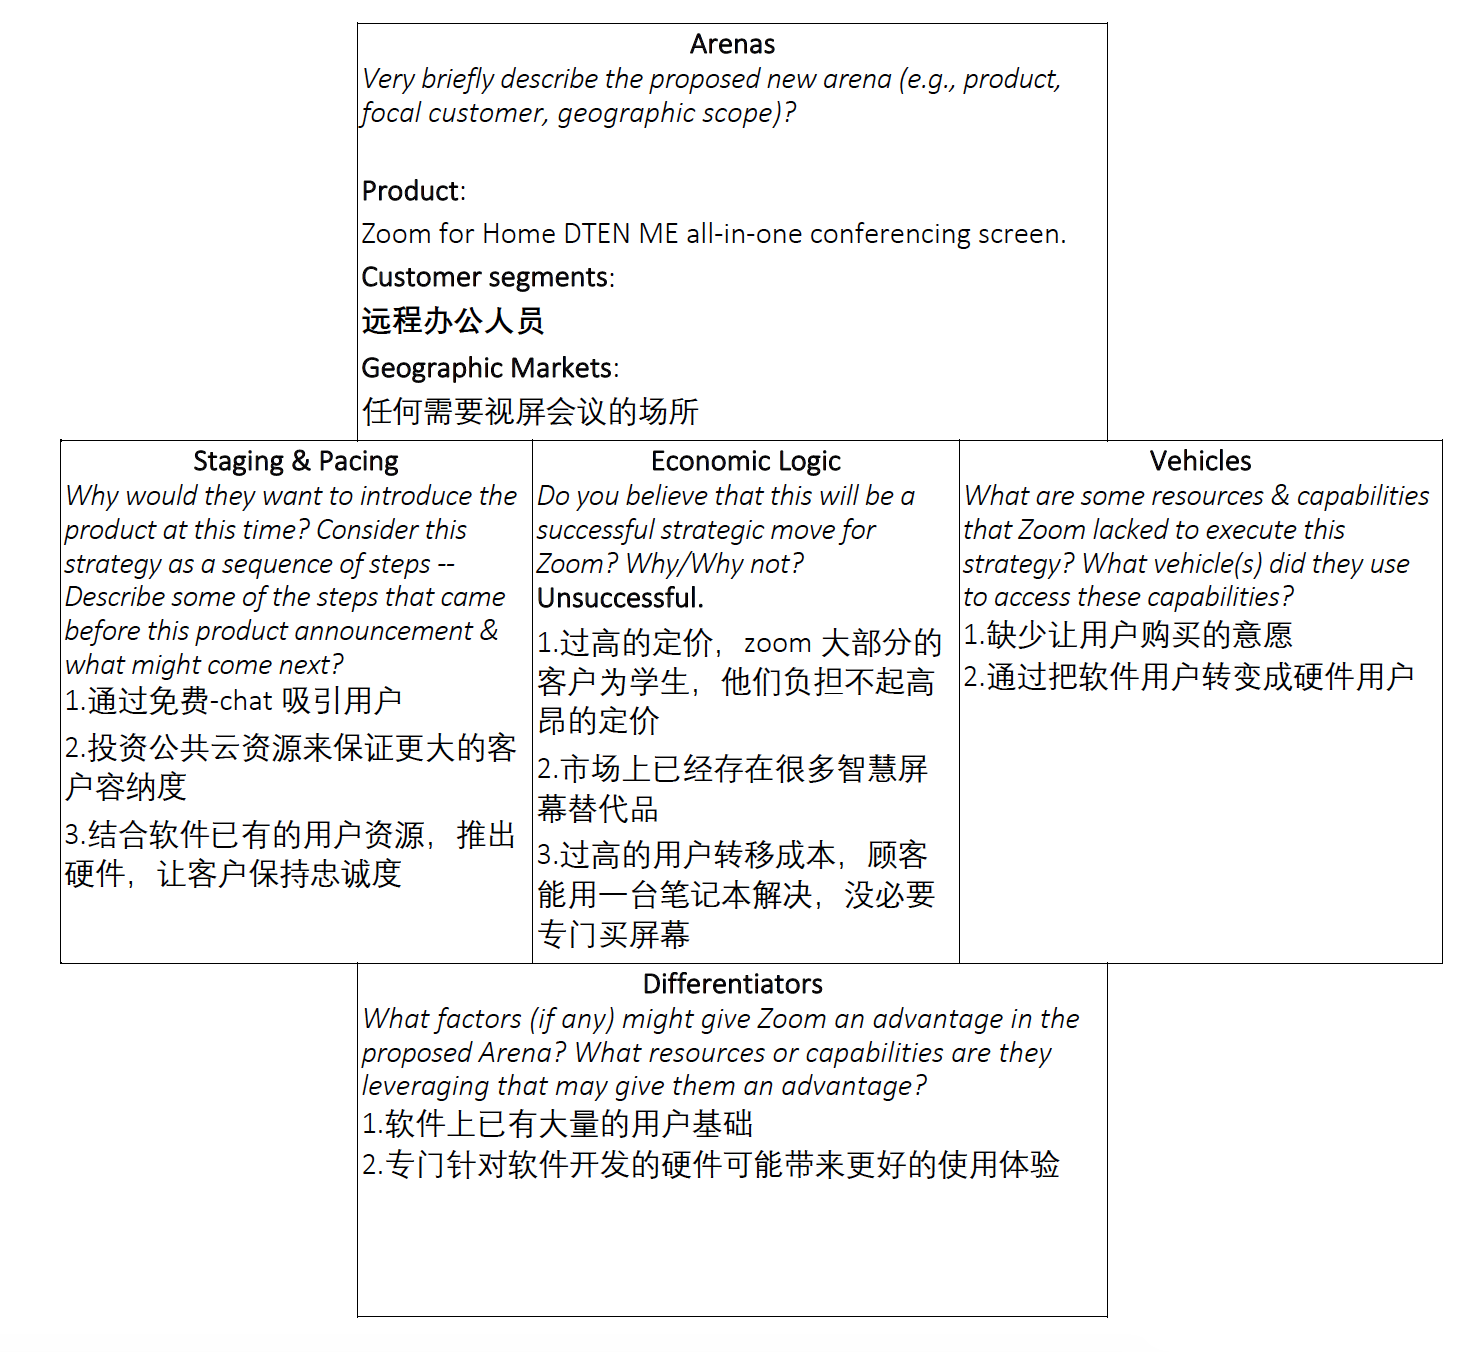
\includegraphics[width=7.5cm]{pics/q1.png}
\end{figure}
\end{frame}


%------------------------------------------------


%------------------------------------------------
\section{Macro Trends/ PESTEL}
\begin{frame}
\frametitle{Macro Trends/ PESTEL}

\begin{block}{Political}
COVID期间实行隔离(Quarantine)政策,封校封城。
\end{block}

\begin{block}{Economic}
宏观经济不景气,线下工作无法展开,失业率上升。
\end{block}

\begin{block}{Sociocultral}
隔离在家人们有社交需求,由于隔离产生新生活方式,线上工作学习社交需求放大。
\end{block}
\end{frame}
%------------------------------------------------
\begin{frame}
\frametitle{Macro Trends/ PESTEL}
\begin{block}{Technological}
信息技术发展,网络设备普及。线上高清实时视频技术成熟。
\end{block}
\begin{block}{Ecological}
居家办公,减少通勤交通产生碳排放。
\end{block}
\begin{block}{Legal}
相关法规出于对用户数据保护对技术服务商进行监察与限制。
\end{block}
\end{frame}

%------------------------------------------------
\section{Industry Analysis}

\begin{frame}
\frametitle{Industry Analysis}
\begin{columns}[c]  %The "c" option specifies centered vertical alignment while the "t" option is used for top vertical alignment

\column{.7\textwidth} % Left column and width

\begin{enumerate}
    \item Was the video conferencing market attractive (pre-COVID)?You could refer the five forces worksheet to make the analysis.
    \item How did the COVID change the market attractiveness?
    \item Evolution: How will the industry change going forward?
\end{enumerate}

\column{.3\textwidth} % Right column and width
% Lorem ipsum dolor sit amet, consectetur adipiscing elit. Integer lectus nisl, ultricies in feugiat rutrum, porttitor sit amet augue. Aliquam ut tortor mauris. Sed volutpat ante purus, quis accumsan dolor.

\end{columns}
\end{frame}

\begin{frame}
\frametitle{Five Forces Sheet (Pre-COVID)}
\begin{figure}[h]
    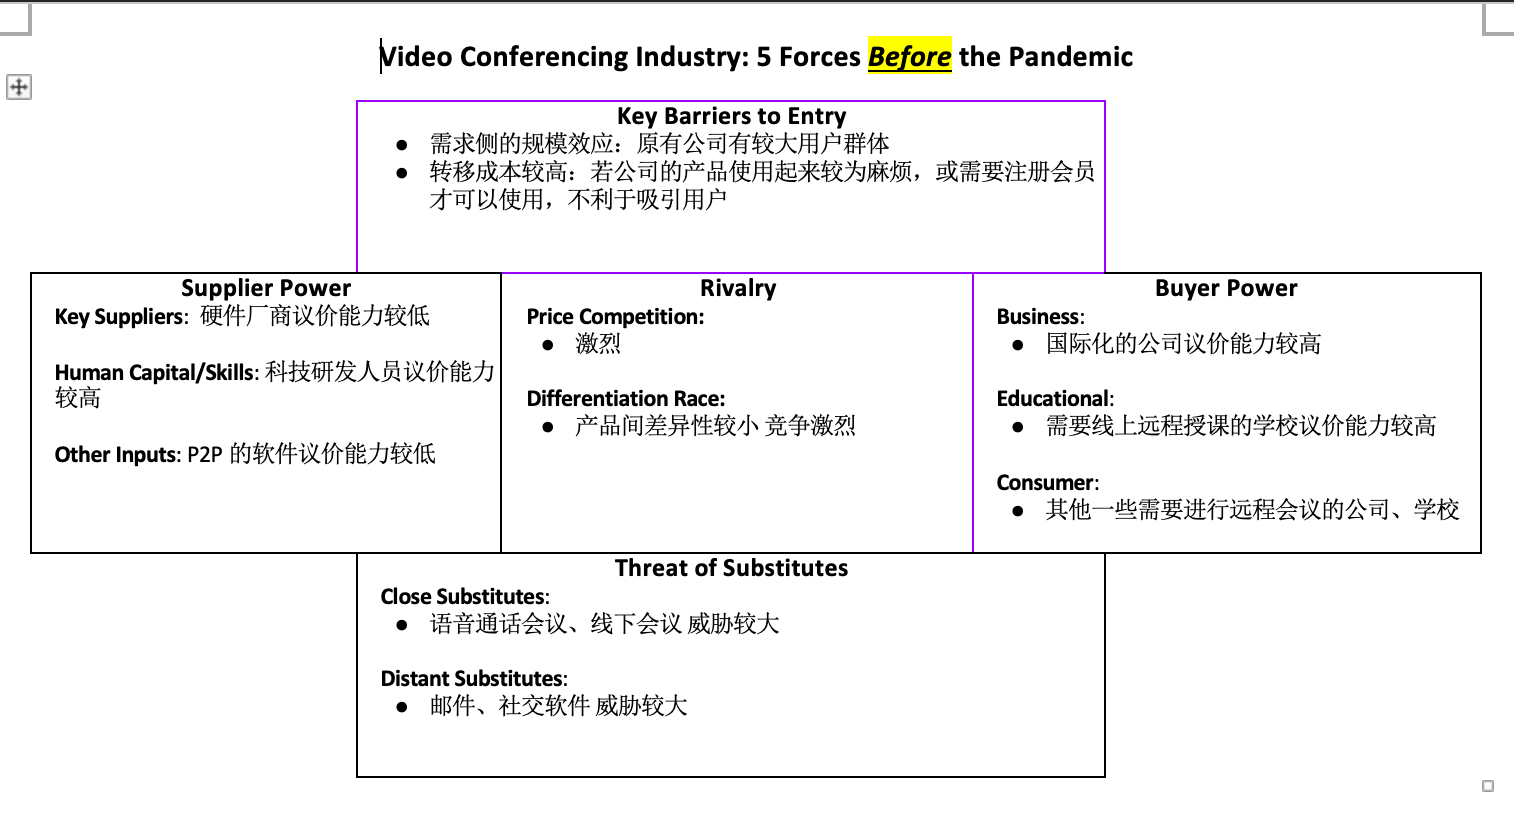
\includegraphics[width=12cm]{pics/before.png}
\end{figure}
\end{frame}

\begin{frame}
\frametitle{Five Forces Sheet (During-COVID)}
\begin{figure}[h]
    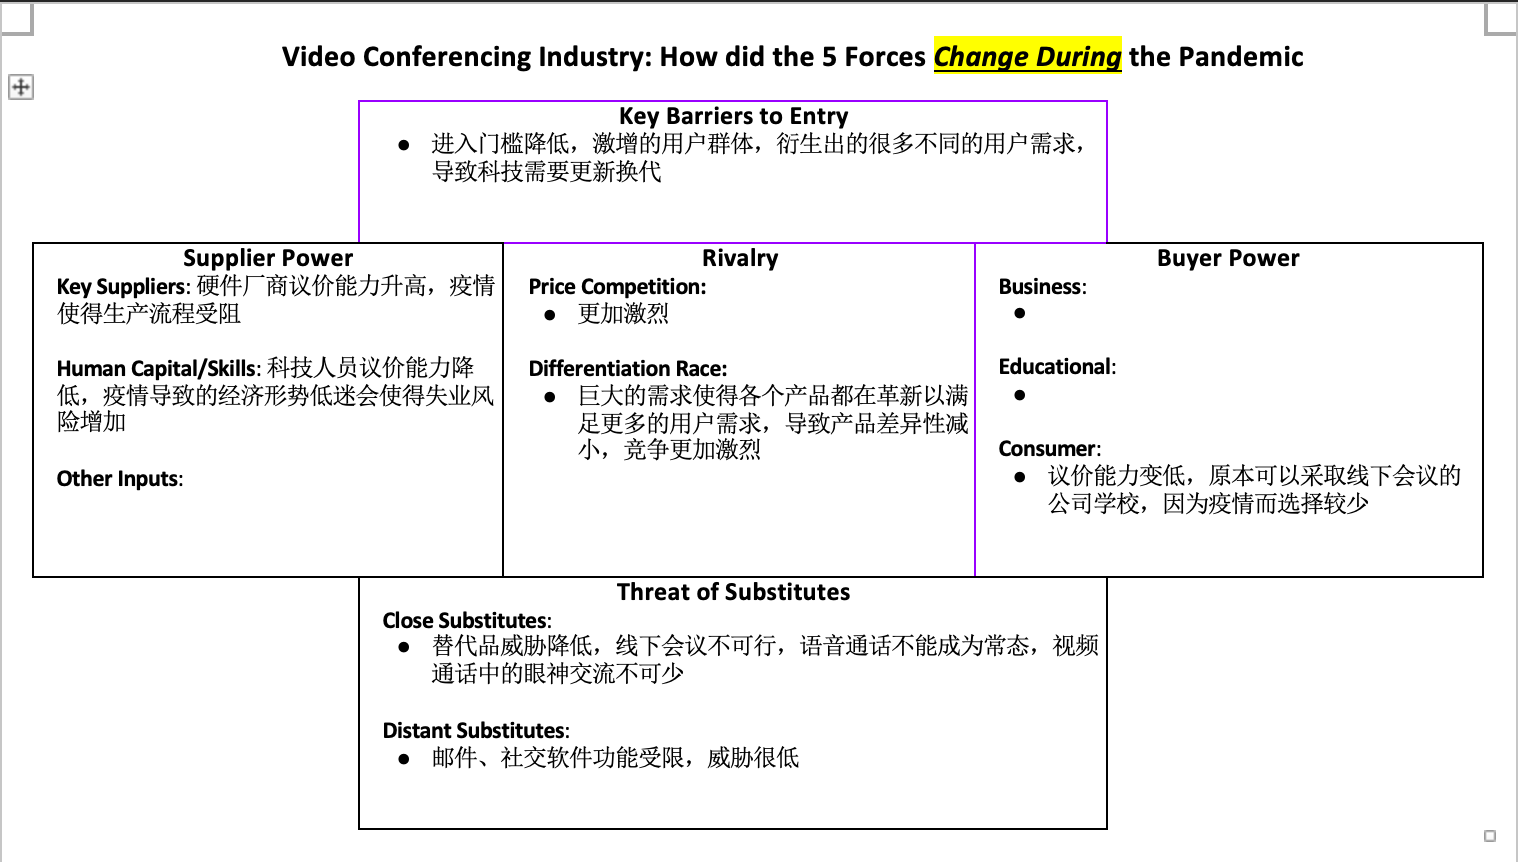
\includegraphics[width=12cm]{pics/during.png}
\end{figure}
\end{frame}

\begin{frame}
\frametitle{Five Forces Sheet (Post-COVID)}
\begin{figure}[h]
    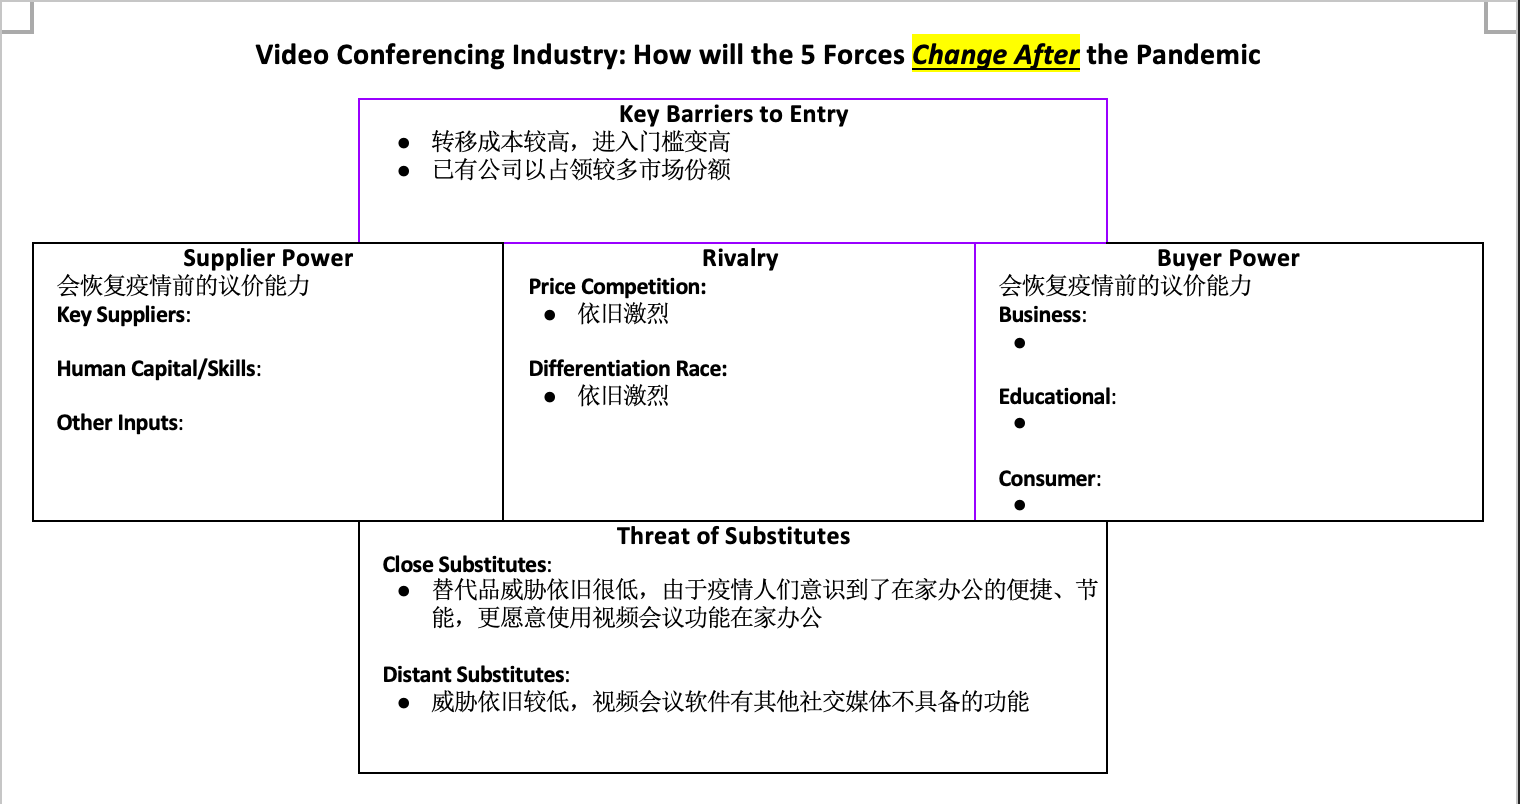
\includegraphics[width=12cm]{pics/after.png}
\end{figure}
\end{frame}

\begin{frame}[allowframebreaks]
\frametitle{Five Forces Sheet (Summary)}
\begin{enumerate}
    \item Key Barriers to Entry
    \begin{itemize}
        \item 拥有大量资源和整合能力及完整生态链的大型互联网公司。例如腾讯,微软等。
        市场红海化,竞争过于激烈,大型互联网公司的主要盈利点及发展点不在视频会议软件服务上,资源的倾斜有限,开发新产品线的必要性不足,用户体验感不足。
        推出的视频会议服务要基于该产业线的生态环境。
        \item 新兴发展的中小型创业公司。
        用户流量不足,难以在前期宣传期吸引客户达到盈利的目的。
        \item 直播等视频平台转型或新开产品线。
        用户服务体验不同,技术支持不足,终端计算能力不强。
        整体进入门槛较低
    \end{itemize}
    \framebreak
    \item Supplier Power
        \begin{itemize}
            \item 硬件服务器端
            几乎没有与其的议价能力,因为硬件服务器端基本上被硬件产品大厂垄断,全球标准基本统一。
            \item 云视频服务费
            原因如上,但是提供云计算的公司还是远大于硬件服务器端的,故而相对来说有一定的议价能力。大量云计算以及服务器公司还是很乐意与zoom这样稳定的产业合作。
            \item 市场营销侧
            Zoom的百分之五十的利润用于获客,这是zoom的战略,在市场营销侧zoom也拥有一定的议价能力,可以替换营销公司。
            \item 技术研发工作外包
            Zoom将大量的技术研发工作外包在杭州等地。这些外包公司的议价权很低,外包公司多,竞争强,zoom本身的强行。
            zoom与供应商侧的整体议价能力较低
        \end{itemize}  
        \framebreak
    \item Rivalry 整体竞争激烈(HighPower)
    \begin{itemize}
        \item Rivals List \begin{enumerate}
            \item Cisco webX
            \item Ringctral
            \item GoToMeeting
            \item 腾讯会议
            \item 钉钉
        \end{enumerate}
        \item \textcolor{blue}{市场份额占比,提供服务是否同质(例如zoom提供单纯的会议场景,而钉钉以及腾讯会议等会提供传输文档等功能,以支持跨行业应用),市场战略区位(主要是全球,北美,中国或是哪里)}    
    \end{itemize}
    
        
    \framebreak
    \item Buyer Power
    \begin{itemize}
        \item Buyer List \begin{enumerate}
            \item 公司
            \item 学校(大学)
            \item 教育机构(补习机构)
        \end{enumerate}
        \item 主要因素:
        \begin{itemize}
            \item 会议频率
            \item 工作/学习时间内的人员流动性
            \item 会议/课程紧迫性
            \item Zoom对于买家的整体议价能力较低
        \end{itemize}
        
        
    \end{itemize}
    \framebreak
    \item Threat of Substitutes
    \begin{itemize}
        \item Substitutes List \begin{enumerate}
        \item 线下会议
        \item 实时通讯工具
        \item 语音会议
        \item 邮件通讯
        \end{enumerate}
        \item 线下会议沟通成本更低,沟通交流的人文关怀以及情感交流更甚。可以知道的是,在商业会议以及课堂应用中,人与人的线下见面交流是具有其不可替代性的。
        语音会议与视频会议一样拥有其便捷性,对于更对无需见面传达的内容来说,语音交流更加便捷,对于技术的支持要求更低,不易出现卡顿。
        邮件通讯是传统且正式的交流方式,对于一些非互联网公司来说,考虑到更多年长的工作人员,这种交流方式具有其不可替代性。        
    \end{itemize}
    \end{enumerate}
\end{frame}
%--------------------------------  

%------------------------------------------------
\section{Resource and Capabilities}
%------------------------------------------------

\begin{frame}[allowframebreaks]
\frametitle{Resource and Capabilities}
\textcolor{blue}{a. What resources and capabilities that make Zoom so successful even before the COVID pandemic? (VRIO Framework)}
\begin{table}
\begin{tabular}{c c c c c}
\toprule
\textcolor{blue}{\textbf{Resource}} & \textbf{V} & \textbf{R} & \textbf{I} & \textbf{O} \\
\midrule
企业文化  & \textcolor{blue}{True} & \textcolor{blue}{True} & \textcolor{blue}{True} & \textcolor{blue}{True}\\
人力资源 & \textcolor{blue}{True} & \textcolor{blue}{True} & \textcolor{blue}{True} & \textcolor{blue}{True}\\
市场决策 & \textcolor{blue}{True} & \textcolor{blue}{True} & \textcolor{red}{False} & \textcolor{red}{False}\\
\bottomrule
\end{tabular}
\caption{VRIO Sheet Before COVID}
\end{table}

%------------------------------------------------


\frametitle{Resource and Capabilities}
% \begin{columns}[c]  %The "c" option specifies centered vertical alignment while the "t" option is used for top vertical alignment
% \column{.5\textwidth} % Left column and width
\begin{enumerate}
    \item 企业文化
    \begin{itemize}
        \item \textbf{V}\quad \textcolor{blue}{True} 
        \begin{itemize}
            \item "Deliver Happiness" 从CEO传递到客户和员工,整体是一个正向反馈。
            \item "Care" 使公司上下人员更有归属感。
        \end{itemize}
        \item \textbf{R/I/O}\quad \textcolor{blue}{True}
    \end{itemize}
    \framebreak
    \item 人力资源
    \begin{itemize}
        \item \textbf{V}\quad \textcolor{blue}{True} 
        \begin{itemize}
            \item \textbf{CEO}的独特经历,\ 了解webex不成功的原因,以及拥有很多用户反馈数据,知道该产业核心痛点。         
            \item 拥有具有强烈归属感以及使命感的优秀\textbf{员工},全员自主热心销售推广。
        \end{itemize}
        \item \textbf{R}\quad \textcolor{blue}{True} \textbf{CEO}的经历独特,稀缺。
        \item \textbf{I}\quad \textcolor{blue}{True} 
        \item \textbf{O}\quad \textcolor{blue}{True} 企业拥有良好的正反馈制度,以保证\textbf{员工}的个人价值发挥到最大。令企业获取更高的效益。
    \end{itemize}
    \item 市场决策
    \begin{itemize}
        \item \textbf{V}\quad \textcolor{blue}{True} 
        \begin{itemize}
        \item 洞察力与前瞻性
        \item 注重用户体验
    \end{itemize} 
        \item \textbf{R}\quad \textcolor{blue}{True}
        \item \textbf{I}\quad \textcolor{red}{False}
        \begin{itemize}
            \item 互联网公司,所有决策很容易被模仿,例如免费体验等措施。
            \item 用户体验的交互设计提升与模仿都很容易
        \end{itemize}
        \item \textbf{O}\quad \textcolor{red}{False}
    \end{itemize}
\end{enumerate}
% \end{column}

%------------------------------------------------


%------------------------------------------------

    \frametitle{Resource and Capabilities}
    \textcolor{blue}{b.	What has Zoom been more effective than rivals during the pandemic ?}
    \begin{table}
    \begin{tabular}{c c c c c}
    \toprule
    \textcolor{blue}{\textbf{Resource}} & \textbf{V} & \textbf{R} & \textbf{I} & \textbf{O} \\
    \midrule
    企业口碑  & \textcolor{blue}{True} & \textcolor{blue}{True} & \textcolor{blue}{True} & \textcolor{blue}{True}\\
    精准定制 & \textcolor{blue}{True} & \textcolor{blue}{True} & \textcolor{red}{False} & \textcolor{red}{False} \\
    公司政策调整 & \textcolor{blue}{True} & \textcolor{red}{False} & \textcolor{red}{False} & \textcolor{red}{False} \\
    \bottomrule
    \end{tabular}
    \caption{VRIO Sheet During COVID}
    \end{table}
    
    %------------------------------------------------
    
    \frametitle{Resource and Capabilities}
    % \begin{columns}[c]  %The "c" option specifies centered vertical alignment while the "t" option is used for top vertical alignment
    % \column{.5\textwidth} % Left column and width
    \begin{enumerate}
        \item 企业口碑
        \begin{itemize}
            \item \textbf{V}\quad \textcolor{blue}{True} 
            之前就有较好的口碑,疫情期间的用户选择倾向较高。
            \item \textbf{R/I/O}\quad \textcolor{blue}{True}
        \end{itemize}
        \framebreak
        \item 精准定制
        \begin{itemize}
            \item \textbf{V}\quad \textcolor{blue}{True} 
            \begin{itemize}
                \item 在疫情期间,满足大型公司企业学校等机构的功能要求,迅速做出改变软件
                \item 扩大和大型公司企业合作
            \end{itemize}
            \item \textbf{R}\quad \textcolor{blue}{True} 
            \item \textbf{I/O}\quad \textcolor{red}{False} 
        \end{itemize}
        \item 公司政策调整 
        \begin{itemize}
            \item \textbf{V}\quad \textcolor{blue}{True} 免费政策推广,使得更多人愿意使用,前期大量的扩展市场。
            \item \textbf{R/I/O}\quad \textcolor{red}{False}
        \end{itemize}
        
    \end{enumerate}
    \framebreak
    % \end{column}
    
    %------------------------------------------------
    

%----------------------------------------------------------------------------------------
    \frametitle{Resource and Capabilities}
    \textcolor{blue}{c.	Will they be able to keep up the rate of development after COVID ?}
    \begin{table}
    \begin{tabular}{c c c c c}
    \toprule
    \textcolor{blue}{\textbf{Resource}} & \textbf{V} & \textbf{R} & \textbf{I} & \textbf{O} \\
    \midrule
    品牌依赖度  & \textcolor{blue}{True} & \textcolor{blue}{True} & \textcolor{red}{False} & \textcolor{red}{False}\\
    \bottomrule
    \end{tabular}
    \caption{VRIO Sheet After COVID}
    \end{table}
    \frametitle{Resource and Capabilities}
    % \begin{columns}[c]  %The "c" option specifies centered vertical alignment while the "t" option is used for top vertical alignment
    % \column{.5\textwidth} % Left column and width
    \begin{enumerate}
        \item 品牌依赖度
        \begin{itemize}
            \item \textbf{V}\quad \textcolor{blue}{True} 
            \begin{itemize}
                \item 增加了企业对于线上办公教学的依赖度,使得产品销售额增加
                \item 将品牌IP由软件转换至硬件,扩大市场(已购入硬件,将持续使用,,即使疫情结束)
            \end{itemize}
            \item \textbf{R}\quad \textcolor{blue}{True}
            \item \textbf{I/O}\quad \textcolor{red}{False}
        \end{itemize}
    \end{enumerate}
    % \end{column}
    \end{frame}
    
    %------------------------------------------------
    
\end{document} 